\section{local systems on natural alternating diagrams}
Suppose we have a braid word $\omega$ then we have the associated natural alternating diagram $(C, \iota', \xi')$ defined in the previous section.

We can associate a quiver $Q$ to the alternating diagram in such a way that :
\begin{itemize}
\item we have one vertex for regions where all hairs are pointing outward/inward
\item for each crossing, we have an arrow from the vertex corresponding to the region where all hairs pointing outward to inward
\end{itemize}

Once we have an alternating strand diagram, we have the associated spectral curve $SC$. Furthermore, we can embedd the underlying undirected graph of the quiver $Q$ in $SC$ in such a way that $SC$ deformation retracts to $Q$(with abuse of notation I will denote this underlying undirected graph as $Q$)(STZ)
Suppose we have a local system on the spectral curve associated with $(C, \iota', \xi')$, then the restricting to $Q$, we get a local system on $Q$. Note that the pullback, induced by the restriction map, between the space of local systems $H^1(SC, \mathbb{C}^*) \rightarrow  H^1(Q,\mathbb{C}^*)$ is an isomorphism.

$H^1(Q,\mathbb{C}^*)$ is isomorphic to $(\mathbb{C}^*)^{|Arr(Q)|}//(\mathbb{C}^*)^{|Vert(Q)|}$
here the group action is defined as the following : let $g_v in (C^*)^{|Vert(Q)|}$
what I mean by $g_v$, only supported at index $v$ with value $g_v$. For other indices the entries are $1$.
then $g_v \cdot (x_a)_{a\in Arr(Q)}$ is 
\begin{itemize}
\item for entries with index $a$ such that the source of $a$ is $v$ i.e. $s(a) = v$, we have $g_v.x_a$
\item for entries with index $a$ such that the target of $a$ is $v$ i.e. $t(a) = v$, we have $g_v^{-1}\cdot x_a$
\end{itemize}


Now we define the associated constructible sheaf on some regular cell complex refinement of the natural alternating strand diagram associated with local systems on $Q$.

First, I will describe the special kind of regular cell complex associated with the alternating strand diagram. 

Suppose we fix a generator region for the alternating strand diagram. Then we label $j^{th}$ crossing(numbering starts from left to right) the $i^{th}$ blue strand(numbering starts from top to bottom) crosses red strands as $c_{i,j}$. We will call the crossing between $i^{th}$ and $i+1^{th}$ red strand as $c$.

Suppose we have an alternating diagram. Then for each crossing $c_{i,j}$ we add 
- two $0$ dimensional strata at the interiors of the $1$ dimensional strata at the northwest(northeast resp.) and southwest(southeast resp.) of the crossing when $j$ is even(odd resp.)
- one $1$ dimensional stratum at the interior of the west region of the crossing connecting the above two $0$ dimensional strata. We will draw this line in a squiggly line
Also for the crossing $c$, we add
- two $0$ dimensional strata at the interiors of the $1$ dimensional strata at the northwest and southwest of the crossing.
 
Below is the picture of a generator region of a natural alternating diagram(figure1), labeling of the crossings(figure2), and its regular cell complex refinement(figure3)
\begin{figure}[H] % Optional: [h] means here, [t] for top, [b] for bottom, [p] for page of floats
    \centering
    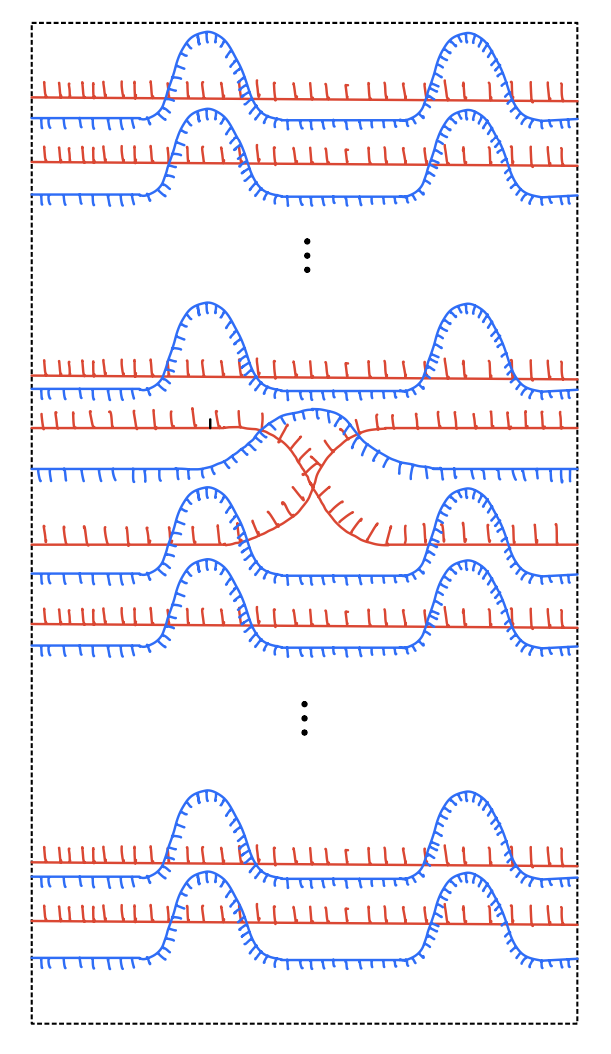
\includegraphics[scale = 0.95]{diagrams/local_systems_on_as_diagrams/1-1.png} % Adjust the width as needed
    \caption{Your caption here}
    \label{fig:your-label}
\end{figure}
\begin{figure}[H] % Optional: [h] means here, [t] for top, [b] for bottom, [p] for page of floats
    \centering
    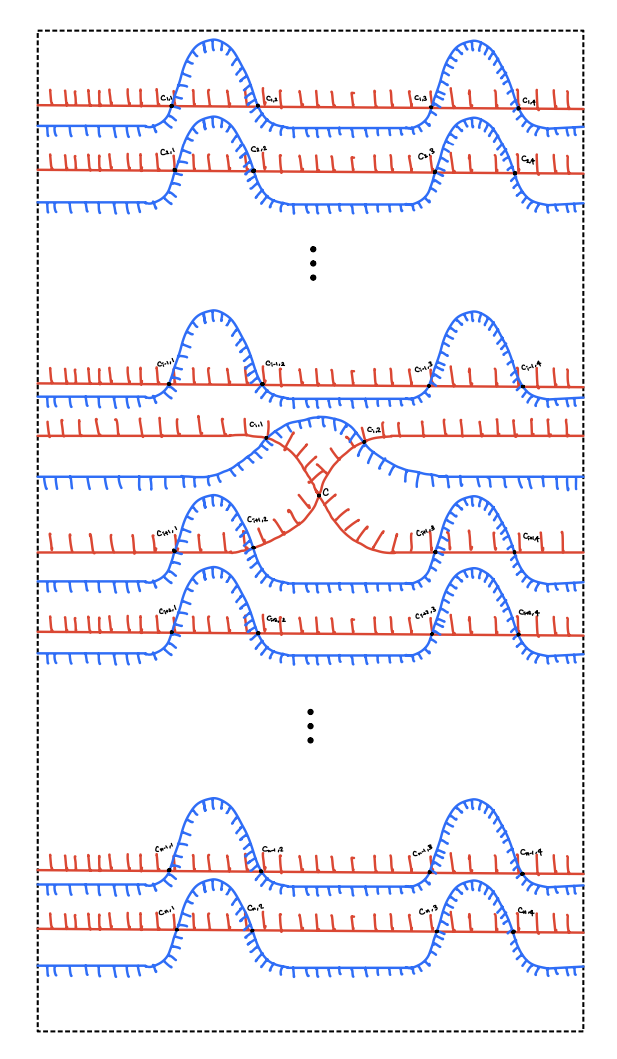
\includegraphics[scale = 0.95]{diagrams/local_systems_on_as_diagrams/1-2.png} % Adjust the width as needed
    \caption{Your caption here}
    \label{fig:your-label}
\end{figure}
\begin{figure}[H] % Optional: [h] means here, [t] for top, [b] for bottom, [p] for page of floats
    \centering
    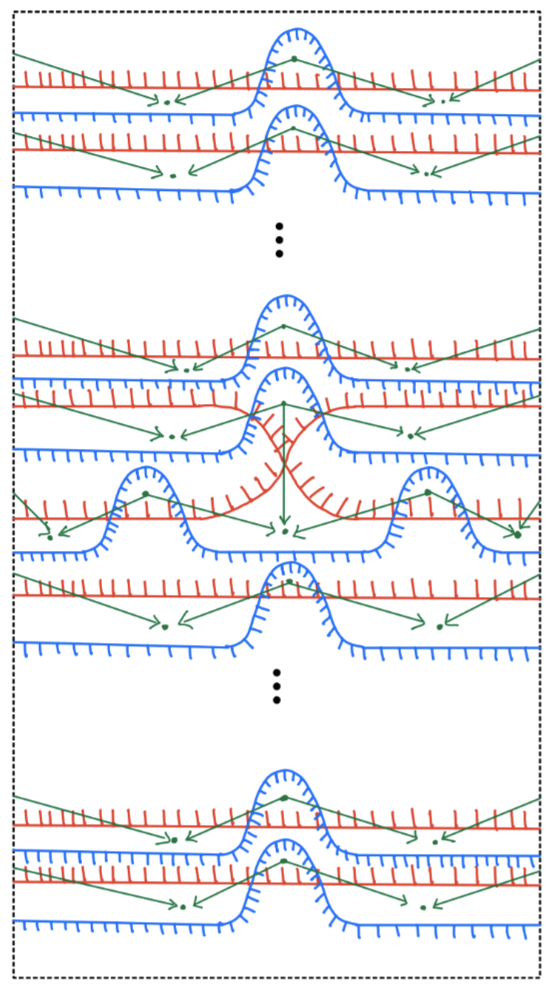
\includegraphics[scale = 0.95]{diagrams/local_systems_on_as_diagrams/2.png} % Adjust the width as needed
    \caption{Your caption here}
    \label{fig:your-label}
\end{figure}


Now I will describe a way to specify a constructible sheaf on the above regular cell complex refinement associated with the local system on $Q$. suppose we have a local system on $Q$ which can be represented as an element of $(\mathbb{C}^*)^{|Arr(Q)|}$:
\begin{enumerate}[label= (\roman*)]
\item stalk of the region where all the hairs are pointing outward is $\mathbb{C}[-1]$
\item stalk of the region where all the hairs are pointing inward is $\mathbb{C}$
\item stalk of the region that has crossing at its boundary and surrounded by a squiggly line is $\mathbb{C}\rightarrow\mathbb{C}$ where the map is multiplication by $g_a$ where $a$ is the arrow goes from the south of the crossing to the north of the crossing
\item the only nonzero genrization maps are region of type (\Rn{3}) to (\Rn{1}) or (\Rn{1}) to (\Rn{2})
\end{enumerate}

In the first case, the map is
\[
  \begin{tikzcd}
    \mathbb{C} \arrow{r}{id} & \mathbb{C} \\
    \mathbb{C}\arrow{u}{} \arrow{r}{}& 0\arrow{u}{}
  \end{tikzcd}
\]
In the latter case, the map is 
\[
  \begin{tikzcd}
	0 \arrow{r}{} & \mathbb{C} \\
    \mathbb{C}\arrow{u}{} \arrow{r}{id}& \mathbb{C}\arrow{u}{}
  \end{tikzcd}
\]

For example, suppose we have a regular cell complex refinement of a generator region and the associated quiver Q as follows:
\begin{figure}[H] % Optional: [h] means here, [t] for top, [b] for bottom, [p] for page of floats
    \centering
    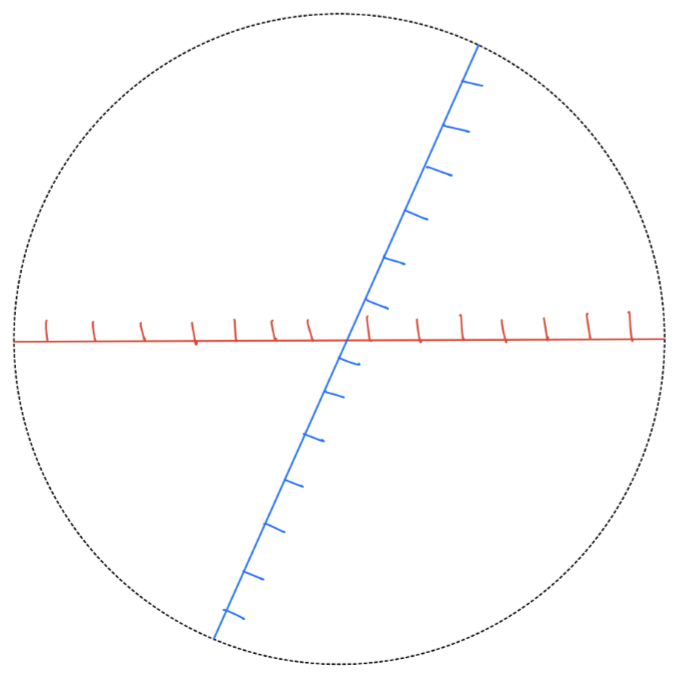
\includegraphics[scale = 0.95]{diagrams/local_systems_on_as_diagrams/3.png} % Adjust the width as needed
    \caption{Your caption here}
    \label{fig:your-label}
\end{figure}

and a local system represented by 
$(g_{a_i})_{a_i\in Arr(Q)}$
then we get the associated constructible sheaf:
\begin{figure}[H] % Optional: [h] means here, [t] for top, [b] for bottom, [p] for page of floats
    \centering
    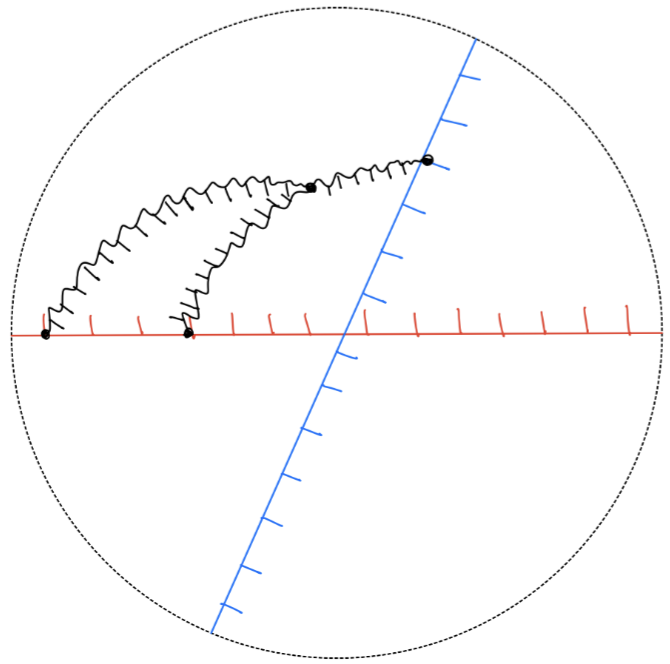
\includegraphics[scale = 0.95]{diagrams/local_systems_on_as_diagrams/4.png} % Adjust the width as needed
    \caption{Your caption here}
    \label{fig:your-label}
\end{figure}

Note that the group action maps a constructible sheaf to the isomorphic constructible sheaf. Therefore, we have a well defined map
$H^1(SC,\mathbb{C}^*)\rightarrow \mathcal{M}_{\overline{(C,\iota',\xi')}}(C)$ where $\overline{(C,\iota',\xi')}$ is the regular cell complex refinement of the natural alternating diagram $(C,\iota',\xi')$.